\chapter{Map Data Sources}\label{chap:mapdatasources}

\textcolor{orange}{Notater:}
hva dette kapittelet er... hvorfor vi trenger data... hvordan vi fikk datakildene... 
Data var VELDIG sentralt i prosjektet, 
\begin{itemize}
    \item Ikke våre data, men de er tilgjengelige åpent, noen under NLOD.
    \item Sammenkoble forskjellige datakilder
\end{itemize}
\textcolor{orange}{ferdig notater}

\section{Map Layers}\label{sec:maplayers}

% KANKJE GLOSSARY FOR "COMPOSITE MAP"
The interactive map on the website supports multiple layers, allowing the user to build a composite map with various types of data. These layers include both meteorological and geological data relevant to assessing road conditions and the surrounding environment.

\subsection{Base Layers}\label{subsec:baselayers}

The user has the option to change the base layer of the map. In the current version, two options are available: the standard map from \Gls{openstreetmap}\footnote{\url{https://www.openstreetmap.org}} and the terrain map from OpenTopoMap\footnote{\url{https://opentopomap.org}}.
% KANSKJE GI GRUNN TIL HVORFOR DET IKKE KUN ER ETT BASE LAYER VALG

\begin{figure}[h]
     \centering
     \begin{subfigure}[b]{0.45\textwidth}
         \centering
         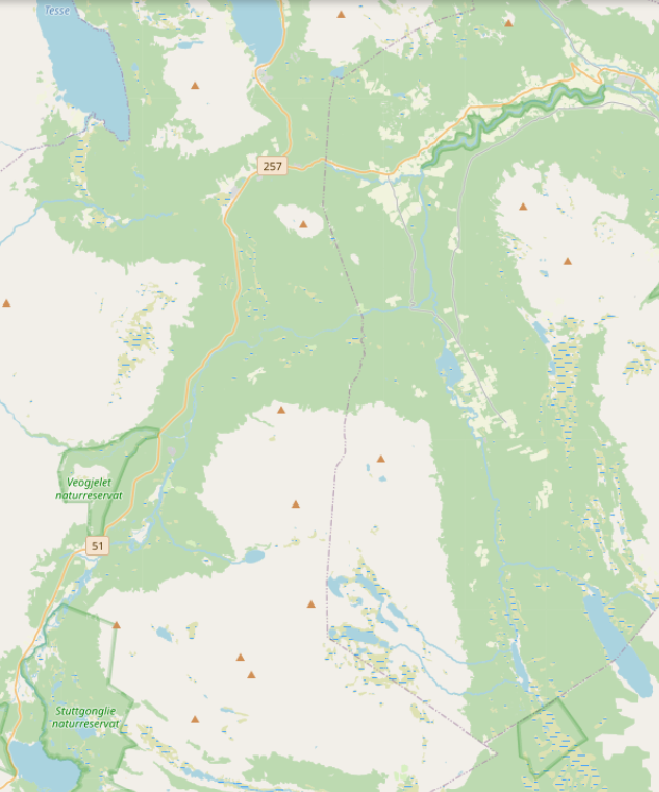
\includegraphics[width=\textwidth]{figures/base_layer_standard.pdf}
         \caption{Standard base layer}
         \label{fig:maplayer:standardlayer}
     \end{subfigure}
     \hfill
     \begin{subfigure}[b]{0.45\textwidth}
         \centering
         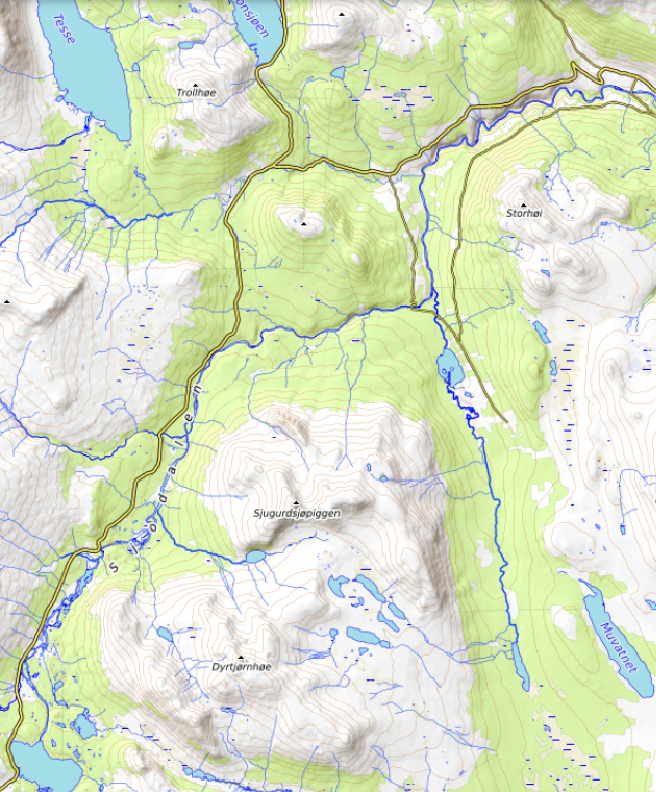
\includegraphics[width=\textwidth]{figures/base_layer_topo.pdf}
         \caption{Terrain base layer}
         \label{fig:maplayers:topolayer}
     \end{subfigure}
    \caption{Base map layer options}
    \label{fig:maplayer:baselayers}
\end{figure}

\subsection{Superficial Deposits}\label{subsec:superficialdeposits}
% LEGGE INN FARGE KODER FOR LØSMASSETYPE. TRENGER IKKE FOR ALLE? KANSKJE VEDLEGG?
The map layer showing superficial deposits is provided by \acrfull{ngu}\footnote{\url{https://www.ngu.no/en}}. The superficial deposits data provide information on the distribution of surface sediments covering bedrock, mainly formed during and after the last Ice Age. It represents the dominant soil type in the upper layers, but does not account for deeper variations. These soil types include stones, gravel, sand, clay, peat, and moraine material \cite{geonorge_losmasser}. 

\begin{figure}[h]
    \centering
    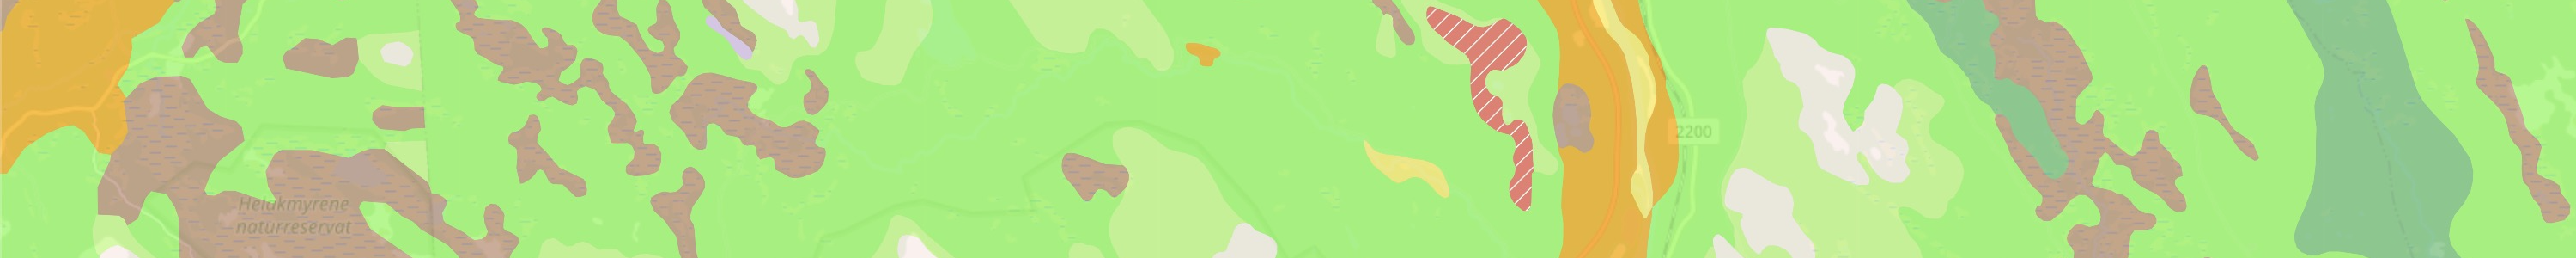
\includegraphics[width=1\linewidth]{images/maplayers/superficialdeposits.png}
    \caption{Example of the superficial deposits map layer}
    \label{fig:maplayer:superficialdeposit}
\end{figure}

\subsection{Frost Depth}\label{subsec:frostdepth}

The frost depth map layer, provided by \acrfull{nve}\footnote{\url{https://www.nve.no/english}}, visualizes frost depth as a raster map, with colors ranging from dark blue (indicating deep frost) to light green (indicating no frost). This layer is particularly useful for assessing the trafficability of forestry roads. When frost depth reaches \qty{10}{\centi\meter} or more (see \autoref{tab:frost_depth_classification}, road conditions are generally suitable for heavy vehicles. As a result, most forestry roads tend to have good trafficability throughout the Norwegian winter, when frost is typically present \cite{wiki:tele}.

% KANSKJE GI EKSEMPLER PÅ NÅR (OG HVOR) DET ER VANLIG MED DE FORSKJELLIGE DYBDENE
\begin{table}[h]
    \centering
    \begin{tabular}{|l|l|l|}
        \hline  
        \textbf{Color} & \textbf{Frost Depth} & \textbf{Depth in cm} \\
        \hline
        \cellcolor[HTML]{00009c} & Very Deep Frost & > 75 cm \\
        \hline
        \cellcolor[HTML]{0018ff} & Deep Frost & 30-75 cm \\
        \hline
        \cellcolor[HTML]{009aff} & Frost & 10-30 cm \\
        \hline
        \cellcolor[HTML]{84ebff} & Shallow Frost & 5-10 cm \\
        \hline
        \cellcolor[HTML]{deffff} & Partially Frost-free & 0-5 cm \\
        \hline
        \cellcolor[HTML]{cef77b} & No Frost & 0 cm \\
        \hline
    \end{tabular}
    \caption[Frost depth classification and corresponding colors]{Frost depth classification and corresponding colors, as defined by \acrshort{nve} \cite{nve2025waterdata}}
    \label{tab:frost_depth_classification}
\end{table}

An example of the frost depth map layer as it appears on the website is shown in \autoref{fig:maplayer:frostdepth}. The dataset spans from 1957 to nine days into the future and represents daily averages measured from 07:00 to 07:00 the following day. The data is presented as a raster grid with a spatial resolution of $1 \times 1$ km. The color-coded visualization enables users to quickly assess ground conditions based on frost depth, as defined in \autoref{tab:frost_depth_classification}. This makes it particularly useful for identifying seasonal and regional variations in frost conditions.

\begin{figure}[h]
    \centering
    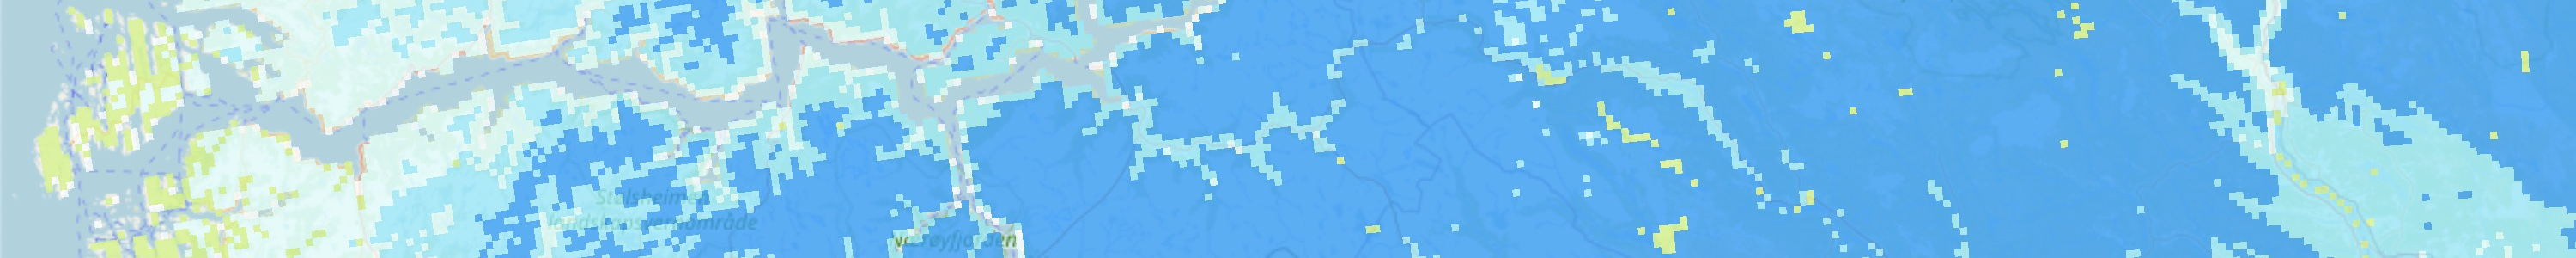
\includegraphics[width=1\linewidth]{images/maplayers/frostdepth.png}
    \caption{Example of the frost depth map layer}
    \label{fig:maplayer:frostdepth}
\end{figure}

\subsection{Soil Saturation}\label{subsec:soilsaturation}

% Glossary groundwater & root zone
The soil saturation data, provided by \acrshort{nve}, represents the ratio between the current simulated water content in the groundwater and root zone and the highest value observed during the historical reference period from 1981 to 2010 \cite{nve2025waterdata}. For example, a soil saturation level of \qty{70}{\percent} indicates that the soil currently holds \qty{70}{\percent} of the maximum water content recorded during that period. An example of how to soil saturation map layer looks like is shown in \autoref{fig:maplayer:soilsaturation}.

\begin{figure}[h]
    \centering
    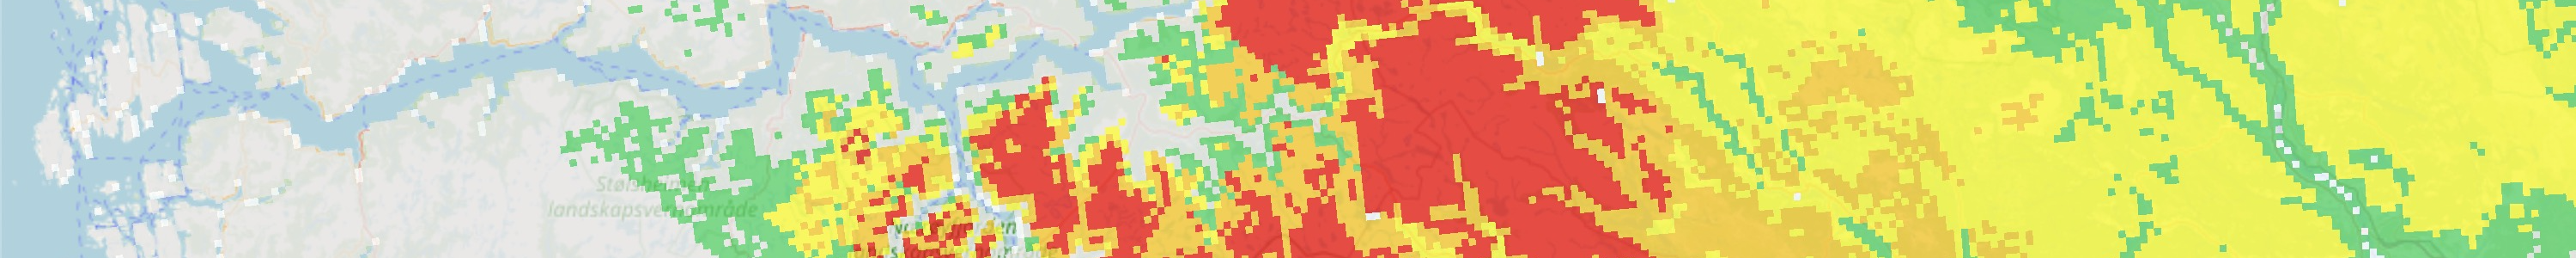
\includegraphics[width=1\linewidth]{images/maplayers/soilmoisture.png}
    \caption{Example of the soil saturation layer}
    \label{fig:maplayer:soilsaturation}
\end{figure}

Soil saturation can be used to assess \gls{trafficability}, which in this context refers to the highest level of soil moisture a road can tolerate without experiencing excessive deformation and potentially lead to dangerous driving conditions. This threshold varies depending on the type of superficial deposits present, as different materials have varying levels of permeability \cite{fjeld2023trafficability}. \acrshort{nve} categorizes soil moisture into distinct levels, as shown in \autoref{tab:soil_saturation_classification}, with the most extreme levels (i.e., the upper percentage range) typically occurring after prolonged rainfall or frost thaw in the spring.

\begin{table}[h]
    \centering
    \begin{tabular}{|l|l|}
        \hline  
        \textbf{Color} & \textbf{Soil Saturation (\%)} \\
        \hline
        \cellcolor[HTML]{f82200} & Above 90\% \\
        \hline
        \cellcolor[HTML]{f8c400} & 80 - 90\% \\
        \hline
        \cellcolor[HTML]{f8fc00} & 70 - 80\% \\
        \hline
        \cellcolor[HTML]{29d460} & 60 - 70\% \\
        \hline
        \cellcolor[HTML]{e4e4e4} & Under 60\% \\
        \hline
    \end{tabular}
    \caption[Soil saturation classification and corresponding colors]{Soil saturation classification and corresponding colors, as defined by \acrshort{nve} \cite{nve2025waterdata}}
    \label{tab:soil_saturation_classification}
\end{table}

\subsection{Forestry Roads}

The forestry roads map layer is the only layer that is altered by the backend server. The backend server uses a vector dataset retrieved via a \Gls{wfs} service in GeoJSON format, provided by GeoNorge\footnote{\url{https://www.geonorge.no/en}} and Kartverket\footnote{\url{https://www.kartverket.no/en}}. In the GeoJSON, forestry roads are represented as geometric LineString features, where each LineString defines a segment between two coordinates. A single road is often divided into multiple such features. The GeoJSON also includes properties of each features such as road number, municipality number, and feature length. An example of how the forestry roads map layer could look like is shown in \autoref{fig:maplayer:forestryroads}.

The backend server alters the GeoJSON by adding additional properties from the other map layers mentioned earlier (\ref{subsec:superficialdeposits}, \ref{subsec:frostdepth}, \ref{subsec:soilsaturation}). In addition to the other map layers, Fjordkatalogen\footnote{\url{https://kartkatalog.miljodirektoratet.no/MapService/Details/fjordkatalogen}} from the Norwegian Environment Agency\footnote{\url{https://www.environmentagency.no/}} is another data source that is used by the Forestry Roads map layer. The implementation of the Forestry Roads service will be explained later in \autoref{chap:implementation}. 

\begin{figure}[h]
    \centering
    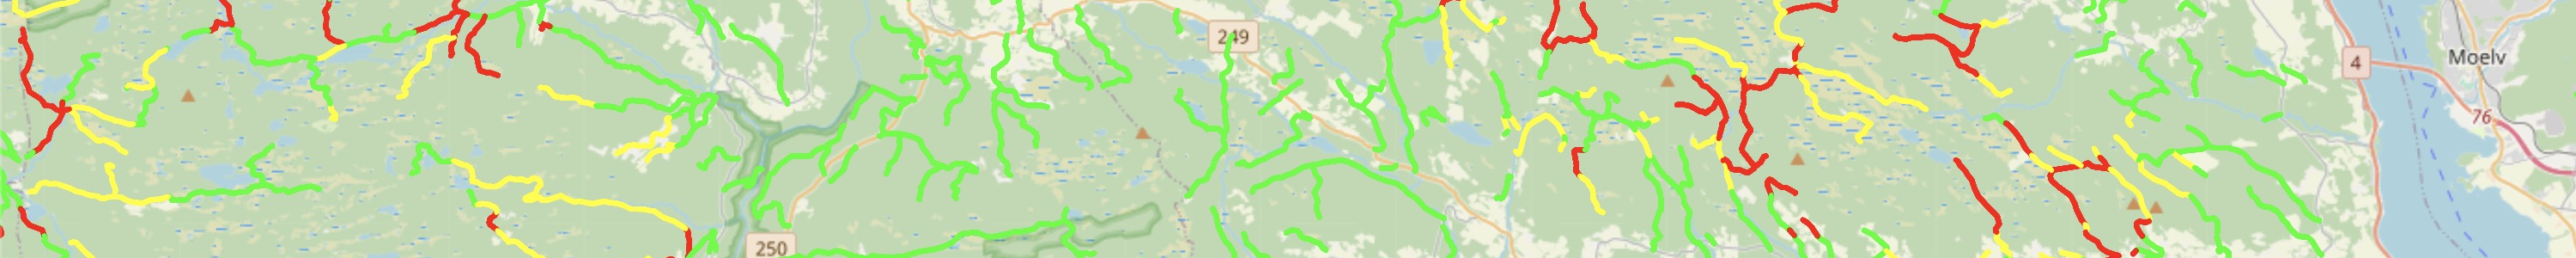
\includegraphics[width=1\linewidth]{images/maplayers/forestryroad.png}
    \caption{Example of the forestry roads map layer}
    \label{fig:maplayer:forestryroads}
\end{figure}

\subsection{Soil Moisture}

Soil moisture is represented as a static raster map indicating areas with the highest likelihood of increased moisture content in the ground. The map highlights zones with a higher risk of deformation of roads and potential impacts on water quality during forestry operations. It is divided into several soil moisture classes, based on the elevation difference (in centimeters) between a given point and the nearest point estimated to be saturated with water. Soil moisture levels are visualized using a graded color scale shown in \autoref{tab:soil_moisture_classification}. The map accounts for surface terrain slope but does not consider superficial deposits \cite{geonorge_soil_moisture}.

\begin{table}[h]
    \centering
    \begin{tabular}{|l|l|}
        \hline  
        \textbf{Color} & \textbf{Soil Moisture (cm)} \\
        \hline
        \cellcolor[HTML]{000080} & Water \\
        \hline
        \cellcolor[HTML]{0000ff} & 0 - 25 cm \\
        \hline
        \cellcolor[HTML]{1e90ff} & 25 - 50 cm \\
        \hline
        \cellcolor[HTML]{00bfff} & 50 - 75 cm \\
        \hline
        \cellcolor[HTML]{87cefa} & 75 - 100 cm \\
        \hline
        \cellcolor[HTML]{ffffff} & > 100 cm \\
        \hline
    \end{tabular}
    \caption[Soil moisture classification and corresponding colors]{Soil moisture classification and corresponding colors, as defined by \acrshort{nibio} \cite{geonorge_soil_moisture}}
    \label{tab:soil_moisture_classification}
\end{table}

The soil moisture layer has a resolution of $1 \times 1$m which makes it especially useful for identifying terrain that is more prone to becoming saturated under wet conditions. When combined with dynamic soil saturation data, it becomes an even more valuable tool, particularly during periods of heavy precipitation or frost thaw. Transport manager can use this map layer to manually inspect the conditions of a potential forestry operation area, by manually checking where increased moisture content could impact the trafficability. An example of the soil moisture layer as visualized in the application is shown in \autoref{fig:soil_moisture_example}.

\begin{figure}[h]
    \centering
    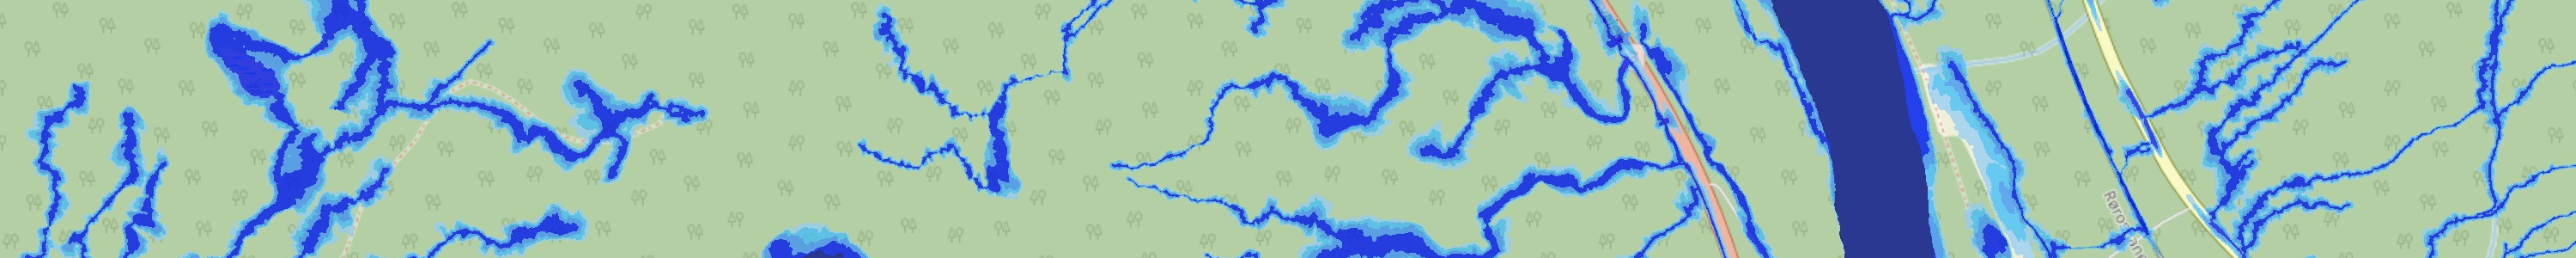
\includegraphics[width=1\linewidth]{images/maplayers/markfuktighet.png}
    \caption{Example of the soil moisture layer}
    \label{fig:soil_moisture_example}
\end{figure}

\section{Gridded Water Balance Model}

The Gridded Water Balance (GWB) model is used to compute hydrological variables displayed on the SeNorge\footnote{\url{https://www.senorge.no}} grid maps. It is a spatially distributed version of the HBV model, originally developed for flood prediction, and calculates the water balance individually for each \qty{1}{\kilo\meter\squared} grid cell \cite{nve2025waterdata}.

Each cell in the grid is defined by its mean elevation and the proportions of various land cover types, such as vegetation, soil, wetlands, lakes, and glaciers. The model runs on a daily basis, using gridded temperature and precipitation data as input \cite{nve2025waterdata}.

The GWB model simulates processes including snow accumulation, moisture in the root zone, groundwater storage, evaporation, surface runoff into rivers, wetlands, and lakes, as well as frost depth and glacier dynamics. Potential evaporation is estimated using air temperature and vegetation growth during the growing season, while actual evaporation depends on the availability of soil moisture \cite{nve2025waterdata}.

Each grid cell’s water balance is calculated independently. Parameters are adapted per cell to account for differences in terrain, vegetation, and soil composition, ensuring that local hydrological behavior is realistically represented \cite{nve2025waterdata}.

The GWB model is also the basis for the frost depth and soil moisture saturation map layers provided by SeNorge and NVE.

\section{Sources of Uncertainty}

\textcolor{orange}{Gjerne skriv om feilkilder fra andre en senorge dataen: SHAPE data (løsmasse, fjord), unøyaktige veidata, }

Various factors contribute to uncertainties in the frost depth and soil saturation maps. These include possible errors in the interpolation of meteorological and soil data, as well as limitations in how the model translates real-world conditions. These uncertainties are especially important around the freezing point (\qty{0}{\celsius}), where even minor temperature variations can influence whether precipitation falls as rain or snow, or if snow begins to melt \cite{senorge_watermap}. The frost depth map tends to provide more accurate simulations of soil freezing compared to soil thawing \cite{nve2025waterdata}.

Localized weather events, such as isolated rain showers missed by nearby weather stations, may also go unnoticed. Furthermore, environmental factors like wind, humidity, and solar radiation, which are not accounted for in the model, can speed up snowmelt, causing discrepancies between the model’s predictions and actual conditions \cite{senorge_watermap}.

The SeNorge maps (frost depth and water saturation) show daily averages, which may miss short-term variations like intense rainfall or rapid changes in temperature within a single day. The forecast maps predict up to nine days ahead, with increasing uncertainty the further into the future the prediction extends. Finally, the model's representation of vegetation and soil types may not always be accurate, potentially leading to the overestimation or underestimation of soil saturation levels \cite{senorge_watermap}.

\section{Unused Data Sources}\label{sec:unuseddatasources}

\textcolor{orange}{Kanskje punktliste istedenfor subsec}

During the preliminary research phase, multiple potential data sources were found in addition to what the ones the Product Owner had knowledge of. \textcolor{orange}{/showed us? personlig så bad}

\subsection{Open-Meteo}

One such potential data source was Open-Meteo\footnote{\url{https://open-meteo.com/}}. Open-Meteo is an open-source weather API that offers free access for non-commercial use \cite{openmeteo}. Open-Meteo offers an expansive range of meteorological data, including historical and forecasts of soil moisture and soil temperature. These variables are central to modeling trafficability \cite{fjeld2023trafficability}, but the spatial resolution of \qty{25}{\kilo\meter\squared} would not give an accurate representation of the conditions in each road. Additional sanity checks of critical periods like thawing and heavy rains suggested that the data could be unreliable. Although Open-Meteo offers great usability and large amounts of data, the spatial resolution and quality of our required data did not meet the application's requirements, and was ultimately left unused. 

\subsection{Satelite Data}

Copernicus som var bra, ettersom det kan si mye om bæreevne (REF DAG FJELD), men hadde for lav oppløsning og var ikke real-time, eller prognose.
\footnote{\url{https://land.copernicus.eu/en/products/soil-moisture}}
\footnote{\url{https://european-flood.emergency.copernicus.eu/en}}

\subsection{Norwegian Meteorological Institute}

Thredds med bra data, men bare 66 timer prognose. Disse hadde mye forskjellige data med høy oppløsning med bra oppløsning
\footnote{\url{https://thredds.met.no/}}
